\documentclass[12pt]{article}

% ---------- PACKAGES ----------
\usepackage[margin=1in]{geometry}     % Set margins
\usepackage{amsmath, amssymb}         % Math symbols
\usepackage{graphicx}                 % Figures
\usepackage{caption}
\usepackage{subcaption}              % Subfigures
\usepackage{hyperref}                % Clickable references
\usepackage{float}                   % Improved float control
\usepackage{booktabs}                % Better tables
\usepackage{siunitx}                 % For SI units
\usepackage{authblk}                 % For multiple authors
\usepackage[backend=biber, style=numeric, sorting=ynt]{biblatex} % Bibliography
\usepackage{tabularx} % In preamble
\usepackage{listings}                % Code
\usepackage{xcolor}
\usepackage{makecell}
\definecolor{codegray}{gray}{0.95}
\definecolor{commentgreen}{rgb}{0,0.6,0}

\lstdefinestyle{pythonstyle}{
    backgroundcolor=\color{codegray},
    commentstyle=\color{commentgreen},
    keywordstyle=\color{blue},
    numberstyle=\tiny\color{gray},
    stringstyle=\color{red},
    basicstyle=\ttfamily\footnotesize,
    breaklines=true,
    captionpos=b,
    keepspaces=true,
    numbers=left,
    numbersep=5pt,
    showspaces=false,
    showstringspaces=false,
    showtabs=false,
    tabsize=4,
    language=Python
}

\addbibresource{references.bib}       % BibTeX file

% ---------- DOCUMENT ----------
\title{Qfolio, a Quantum-based and calsscial NUmpy-based sovler for portfolio optimization package: Benchmark analysis}
\author[1]{Po-Chih Chou}
%\affil[1]{Department of Aerospace Engineering, University of Michigan}

\date{\today}

\begin{document}

\maketitle

\tableofcontents
\newpage

\begin{abstract}

This research investigates the performance of quantum versus classical portfolio optimization methods under varying market conditions and investment strategies. Specifically, we compare a classical NumPy-based solver with the Quantum Approximate Optimization Algorithm (QAOA), implemented via IBM's Qiskit framework, with classical post-processing supported by CPLEX.

The study considers both bull and bear markets, analyzing how solver performance varies with different risk-aversion parameters and capital deployment strategies. We implement binary encoding techniques, inspired by prior work from D-Wave \cite{dwave_portfolio} and IBM Qiskit Finance \cite{qiskit_portfolio}, to map the discrete portfolio selection problem onto a quantum-amenable format.

To ensure realism and benchmarking relevance, we use the Vanguard S\&P 500 ETF (VOO) \cite{Vanguard_VOO} as the target index, comparing it against optimized portfolios composed of its top holdings—AAPL, MSFT, and AMZN. Simulations are limited to four assets due to quantum memory constraints but cover both fixed-capital and incrementally invested portfolios.

Our results show that QAOA consistently outperforms classical optimization by achieving higher returns in bull markets and incurring smaller losses in bear markets, particularly when using low risk-aversion settings. This work highlights QAOA’s potential in practical, real-world financial optimization and lays a foundation for future scaling on quantum hardware.

\end{abstract}

\textbf{Keywords:} Portfolio Optimization, Quantum Algorithm, Quantum Annealing, Quantum Approximate Optimization Algorithm (QAOA). Quadratic Unconstrained Binary Optimization (QUBO).

\section{Introduction}

Portfolio optimization has long been a central and challenging problem in finance. Whether one is an institutional asset manager or an individual investor, the objective remains consistent: maximizing expected returns while managing risk within a given set of constraints. The fundamental theory behind portfolio optimization has been widely studied, and classical formulations, such as those outlined by Ahmed~\cite{ahmed2002optimization}, serve as the foundational framework for many practical applications.

Beating market indices such as the Vanguard S\&P 500 ETF (VOO)~\cite{Vanguard_VOO} remains an enduring goal. Since future price movements are inherently uncertain, investors must rely on historical data to construct strategies that are profitable over defined horizons—ranging from days to years. This motivates the need for robust, data-driven optimization techniques that can adapt to different market conditions.

This paper benchmarks classical and quantum optimization methods to evaluate the practical potential of quantum computing in portfolio construction. While quantum computing offers a broad range of applications, portfolio optimization is a particularly compelling use case due to its combinatorial structure and computational complexity. Investors may adopt different philosophies—such as technical or fundamental analysis—but portfolio allocation is a shared concern across strategies.

Recent advances in quantum computing have enabled the development of algorithms to tackle NP-hard problems, such as the Quantum Approximate Optimization Algorithm (QAOA). To leverage this for portfolio selection, we formulate the optimization problem as a Hamiltonian and solve it using both classical and quantum approaches. The mathematical formulation and algorithmic implementation are discussed in detail in the Methodology section.

Although our study is grounded in a simplified framework, it highlights the potential for quantum algorithms to enhance traditional optimization pipelines. For tractability, we restrict the problem to binary decision-making and assume whole-share allocation, thereby excluding fractional investments. The combinatorial optimization methods discussed here also generalize to other domains such as logistics, supply chain management, scheduling, chemical discovery, and healthcare.


\section{Methodology}

We explore our portfolio optimization problem by following the mean-variance portfolio optimization model for $n$ assets. The main focus of this paper is to benchmark the performance of a classical numerical solver versus a quantum algorithm in solving an NP-hard combinatorial problem. In many cases, exhaustive search is not tractable. Therefore, this paper demonstrates the performance of a quantum algorithm and its potential to outperform traditional computing approaches—especially as quantum computing becomes more accessible and stable.

A basic optimization problem can be formulized as the following 

\begin{equation}
    \begin{array}{ll}
        \text{minimize or maximize} & \text{objective function}\\
        \text{subject to} & \text{constraint(s)}
    \end{array}
\end{equation}

Here, our objective function is to minimize the risk and maximize the return, and the constraint is the budget. There are three main components in our model: 

1.  The decision variable.

2.  The constraints.

3.  The objective function quantifies the criteria of choosing the best decision. 

\subsection{Hamiltonian formulation}

In this section, we will introduce how to convert our problem into a Hamiltonian form which is a energy function defines the total energy $H$ of a given spin configuration.

\begin{equation}
    H = -J\sum_{i,j}s_{i}s_{j} - h\sum_{i}s_{i}
\label{eq:Hamiltonian}
\end{equation}

where $s_{i} \pm 1$ is the spin at site $i$, $J$ is the coupling constant which describese the interaction strength between neighboring spins, $\sum_{i,j}$ is the sum over neighboring pairs, $h$ is the external magnetic field. 

Let's first consider using the index $i$ to denote a particular stock, with an average period return per dollar spent of $r_{i}$ for each stock $i$. Let $\sigma_{i,j}$ be the covariance of returns of stocks $i$ and $j$. For a spending budget of $B$ dollar. We can formulate our problem as following:

\begin{equation}
\begin{aligned}
\text{min} \quad & \sum_{i=1}^{n}\sum_{j=1}^{n} \sigma_{ij}x_{i}x_{j} - \sum_{i=1}^{n} \overline{r_{i}} x_{i}\\
\text{s.t.} \quad &\sum_{i=1}^{n} x_{i} \leq B, \\
            & x_{i} \geq 0, \quad \text{for } i \in \{1, \dots, n\}.
\end{aligned}
\label{eq:base formula}
\end{equation}

where $B$ is the total budget, $R$ is the total return, $\overline{r_{i}}$ is the expected return of our investment. For example, if we choose $n=3$ and we want our return in a given time to be 100 dollars, our decision vriables must satisfied 

\begin{equation}
\sum_{i=1}^{n=3} x_{i} \leq B,\ x_{i}\geq 0.
\end{equation} 

and 
\begin{equation}
    \sum_{i=1}^{n=3} \overline{r_{i}}x_{i} \geq 100,\ x_{i}\geq 0.
\end{equation} 

The values of the decision variables that maximize or minimize the objective function is the best among the set of decision values defined by the constraints in the optimization model. In our example, the objective function is the risk level of the investment.

Next, let's expand our example to let $x_{i}$ denote the number of shares of stock $i$ purchased at price $p_{i}$. We have 

\begin{equation}
    \begin{aligned}
    \text{min} \quad  & \sum_{i=1}^{n}\sum_{j=1}^{n} \sigma_{ij}p_{i}x_{i}p_{j}x_{j} - \sum_{i=1}^{n} \overline{r_{i}} p_{i}x_{i}  \\
    \text{s.t.} \quad  &\sum_{i=1}^{n} p_{i}x_{i} \leq B, \\
                & x_{i} \geq 0, \quad \text{for } i \in \{1, \dots, n\}.
    \end{aligned}
    \label{eq:base formula2}
\end{equation}

From equaiton \ref{eq:base formula2}, we construct our Hamiltonian model in \ref{eq:Hamiltonian} as 

\begin{equation}
    \begin{aligned}
    \min \quad & J(\sum_{i=1}^{n}\sum_{j=1}^{n} \sigma_{ij}p_{i}x_{i}p_{j}x_{j}) - h( \sum_{i=1}^{n}\overline{r_{i}} p_{i}x_{i}),  \\
    \text{s.t.} \quad &\sum_{i=1}^{n} p_{i}x_{i} \leq B, \\
    & x_{i} \geq 0, \quad \text{for } i \in \{1, \dots, n\}.
    \end{aligned}
\label{eq:Form Hamiltonian}
\end{equation}

You may notice $p_{i}x_{i}$ in \ref{eq:Form Hamiltonian} need some adjustment to be apply to keep our decision variale limit to $x_{i}$ seen in \ref{eq:base formula}, otherwise, our problem will not be quadratic anymore, which hinder us to our final goal - Quadratic Unconstrained Binary Optimization formalize (QUBO).

Therefore, we will introduce a technique called binary encoding in the next section to help us.

\subsection{Binary Encoding}

To better reflect real-world investment scenarios, we aim to determine the number of shares $s_i$ for each asset $i$ (with unit price $p_i$), without introducing additional continuous variables, in order to preserve the quadratic form of our optimization problem.

To achieve this, we adopt a binary encoding scheme. Each integer share variable $s_i$ is represented via binary expansion:

\begin{equation}
s_i = 2^{0}x_{i,0} + 2^{1}x_{i,1} + 2^{2}x_{i,2} + \cdots + 2^{m-1}x_{i,m-1},
\end{equation}

where $x_{i,j} \in \{0,1\}$ are binary decision variables, and $m$ is the number of binary bits required to represent the maximum allowable value of $s_i$. For instance, if the maximum number of shares is 5, then $m = 3$ suffices, yielding encodings such as: 0 = 000, 1 = 001, 2 = 010, ..., 5 = 101. This binary formulation enables us to model realistic discrete asset quantities while maintaining compatibility with QUBO (Quadratic Unconstrained Binary Optimization) formulations.

Using this encoding, we reformulate our original problem (refer to Equation~\ref{eq:base formula2}) as:

\begin{equation}
\begin{aligned}
\min_{s_1, \dots, s_n} \quad & \sum_{i=1}^{n} \sum_{j=1}^{n} \sigma_{ij} s_i s_j  - \sum_{i=1}^{n} \overline{r_i} s_i\\
\text{s.t.} \quad & \sum_{i=1}^{n} s_i \leq B, \\
& s_i \geq 0, \quad \text{for all } i \in \{1, \dots, n\}.
\end{aligned}
\label{eq:binary encoded}
\end{equation}

After solving the binary-encoded problem, we decode the optimal values of $s_i$ from the binary solution variables $x_{i,j}$.

Now, let's make this form \ref{eq:binary encoded} into a QUBO form. First, we use $\lambda_{1}$ and $\lambda_{2}$ to denote penalty parameters for our QUBO objective function, respectively.

\begin{equation}
H = q(\sum_{i=1}^{n}\sum_{j=1}^{n} \sigma_{ij}p_{i}x_{i}p_{j}x_{j}) + \lambda_{1}(\sum_{i=1}p_{i}x_{i} - B)^{2} - \sum_{i=1}^{n}\overline{r_{i}} p_{i}x_{i}
\label{eq:QUBO_0}
\end{equation}

Then, by implementing the binary encoding, we can reformulate above Hamiltonian equation \ref{eq:QUBO_0} into QUBO form as 

\begin{equation}
H = q(\sum_{i=1}^{n}\sum_{j=1}^{n} \sigma_{ij}s_{i}s_{j}) + \lambda_{1}(\sum_{i=1}s_{i} - B)^{2} - \sum_{i=1}^{n}\overline{r_{i}} s_{i}
\label{eq:QUBO_binary_encoded}
\end{equation}

where $s_i$ is the enceded binary decision vaeiable. Again, our objective function becomes a quadratic function, technically, a Quadratic Unconstrained Binary Optimization (QUBO) problem.

An important implementation detail lies in the selection of $m$, the number of binary bits used per asset. This determines the upper bound on share quantity and is computed as:

\begin{equation}
m = \left\lceil \log_2\left( \frac{B}{\min(p_i)} \right) \right\rceil, \quad \text{for } i \in \{1, \dots, n\},
\label{eq:num_bits}
\end{equation}

where $B$ is the total investment budget, $p_i$ is the price of asset $i$, and $\lceil \cdot \rceil$ denotes the ceiling function. This guarantees that the encoded variable $s_i$ can span from 0 to the maximum number of affordable shares given budget $B$ and asset prices.


\subsection{Solving the model with classic optimizer}
For the NumPy-Based solver, we have choosen solver package from \texttt{qiskit algorithms}, which includes \texttt{NumPyMinimumEigensolver} \cite{Qiskit_Algorithms_API}. And for the and optimization solver, we use \texttt{MinimumEigenOptimizer} from \texttt{qiskit optimization} \cite{Qiskit_Optimization_API}. This MinimumEigenOptimizer provides a wrapper for the qiskit optimization module to use. The resulting QUBO is then translated into an Ising Hamiltonian whose minimal eigen vector and corresponding eigenstate correspond to the optimal solution of the original optimization problem. The provided minimum eigen solver is then used to approximate the ground state of the Hamiltonian to find a good solution for the optimization problem. By converting our problem into QUBO form in \ref{eq:QUBO_binary_encoded}, we already satisfy the QUBO form and thus reduce the time to convert it. 

\begin{lstlisting}[style=pythonstyle, caption={NumPy-based solver}]
    # NumPy-Based classic solver
    classical_algorithm = NumPyMinimumEigensolver()
    classical_eigensolver = MinimumEigenOptimizer(classical_algorithm)
    print(" --- Solving: Classic solver --- ")
    results = classical_eigensolver.solve(qp)
\end{lstlisting}

\subsection{Solving the model with  Quantum Approximate Optimization Algorithm (QAOA)}

For the Quantum Approximate Optimization Algorithm (QAOA), we employ the same high-level solver interface provided by \texttt{qiskit optimization} \cite{Qiskit_Optimization_API} and the quantum algorithm implementation from \texttt{qiskit algorithms} \cite{Qiskit_Algorithms_API}. QAOA is a variational quantum algorithm designed to approximate solutions to combinatorial optimization problems by minimizing the expectation value of a cost Hamiltonian over a parametrized quantum circuit. In our implementation, we configure the QAOA ansatz with a depth of three repetitions and optimize the variational parameters using the \texttt{COBYLA} classical optimizer with a maximum of 250 iterations. The resulting QAOA instance is wrapped in a \texttt{MinimumEigenOptimizer} to allow for integration with Qiskit's optimization problem workflow. The problem, already in QUBO form as defined in Equation~\ref{eq:QUBO_binary_encoded}, is internally translated into an Ising Hamiltonian, and the QAOA algorithm is used to approximate its ground state, corresponding to a near-optimal solution.

\begin{lstlisting}[style=pythonstyle, caption={QAOA solver}]
    # QAOA solver
    qaoa_optimizer = COBYLA(maxiter=250)
    qaoa_sampler = QAOA(sampler=Sampler(), optimizer=qaoa_optimizer, reps=3)
    qaoa_res = MinimumEigenOptimizer(qaoa_sampler)
    print(" --- Solving: Quantum solver (QAOA) --- ")
    results = qaoa_res.solve(qp)
\end{lstlisting}


\section{Discussion}
\subsection{Benchmark stock \& ETF Selection}
In our data collection, we selected the top four holdings in the VOO ETF: \texttt{AAPL}, \texttt{NVDA}, \texttt{MSFT}, and \texttt{AMZN} \cite{Vanguard_VOO}.

To leverage computational resources and benchmark both classical and quantum algorithms, we implemented a NumPy-based classical solver and the QAOA (Quantum Approximate Optimization Algorithm) implementation in Qiskit. All quantum simulations were executed locally using the Qiskit Aer simulator. The system specifications are as follows: AMD Ryzen 9 6900HS CPU @ 3.30GHz, 16.0 GB RAM, 64-bit OS with x64-based architecture. The environment is configured with \texttt{Python 3.11}, \texttt{Qiskit Algorithms 0.3.1}, and \texttt{Qiskit Optimization 0.6.1}.

One may question the exclusion of \texttt{NVDA} in favor of using \texttt{AAPL}, \texttt{MSFT}, and \texttt{AMZN}. In our initial benchmarking, we aimed to balance computational load, visualization clarity, and memory usage. As of 2023-03-22, \texttt{NVDA}'s adjusted closing price was \$26.45, significantly lower compared to \texttt{AAPL} at \$156.25, \texttt{MSFT} at \$268.03, and \texttt{AMZN} at \$98.70.

Applying Equation~\ref{eq:num_bits} with a budget of \$10{,}000 USD, the resulting number of items ($m_i = \lceil \log_2(B / p_i) \rceil$) would be 8.56 for \texttt{NVDA}, 6.00 for \texttt{AAPL}, 5.22 for \texttt{MSFT}, and 6.66 for \texttt{AMZN}. Consequently, the number of bits needed to encode each decision variable is $m_{\{\text{AAPL, MSFT, AMZN}\}} = 7$ and $m_{\{\text{AAPL, NVDA, AMZN}\}} = 9$. Unfortunately, a register size of $m = 9$ exceeds the feasible memory limits of our local Qiskit Aer simulator for QAOA. Moreover, greater bit depth substantially increases circuit complexity and simulation time. Therefore, we chose the asset subset \{\texttt{AAPL}, \texttt{MSFT}, \texttt{AMZN}\} to balance performance and tractability.

\subsection{Rebalancing Portfolio for a Given Period}

This study incorporates a realistic investment scenario with rebalancing and periodic contributions. Rebalancing occurs at discrete intervals using the closing price on each rebalance date, ensuring that the total portfolio value remains unchanged before and after reallocation. Returns are calculated relative to the portfolio value on the first rebalance date.

For example, if the initial investment date is 2025-01-02, the model uses adjusted closing prices from the five prior trading days (2024-12-24, 2024-12-26, 2024-12-27, 2024-12-30, and 2024-12-31) to estimate expected returns and generate an initial allocation. On the subsequent rebalance date, 2025-01-09, the model again uses the five most recent trading days (2025-01-02 through 2025-01-08) to update portfolio weights. This process continues across all rebalance periods within the evaluation window.

\subsection{Bull market - 2023-10-27 to 2024-10-24}

According to the definition from \cite{fidelity_bear_bull}, a bull market is identified when the market rises at least 20\% from a previous low. We define the bull period using the ETF VOO, which rose from \$367.131 on 2023-10-27 to \$527.310 on 2024-10-24 — a total increase of 40.63\%. Using a rebalancing frequency of every 21 business days, we generated the following schedule. The subsequent analysis also uses a 21-day lookback window for historical return estimation. The optimization is performed with a training period of 21 prior trading days, a rebalance interval of 21 days, and a penalty parameter of \(\lambda_1 = 1000\).

\begin{table}[H]
\centering
\caption{Portfolio Rebalancing Schedules}
\begin{tabular}{|l|p{4cm}|p{5cm}|}
\hline
\textbf{Rebalancing Frequency} & \textbf{Description} & \textbf{Rebalancing Dates} \\
\hline
Every 21 business days & \makecell[l]{Monthly\\rebalancing} & 
\makecell[l]{
2023-10-27, 2023-11-28,\\
2023-12-28, 2024-01-30,\\
2024-02-29, 2024-04-01,\\
2024-04-30, 2024-05-30'\\
2024-07-01, 2024-07-31,\\
2024-08-29, 2024-09-30
} \\
\hline
\end{tabular}
\label{tab:bull_VOO}
\end{table}

\begin{figure}[H]
    \centering
    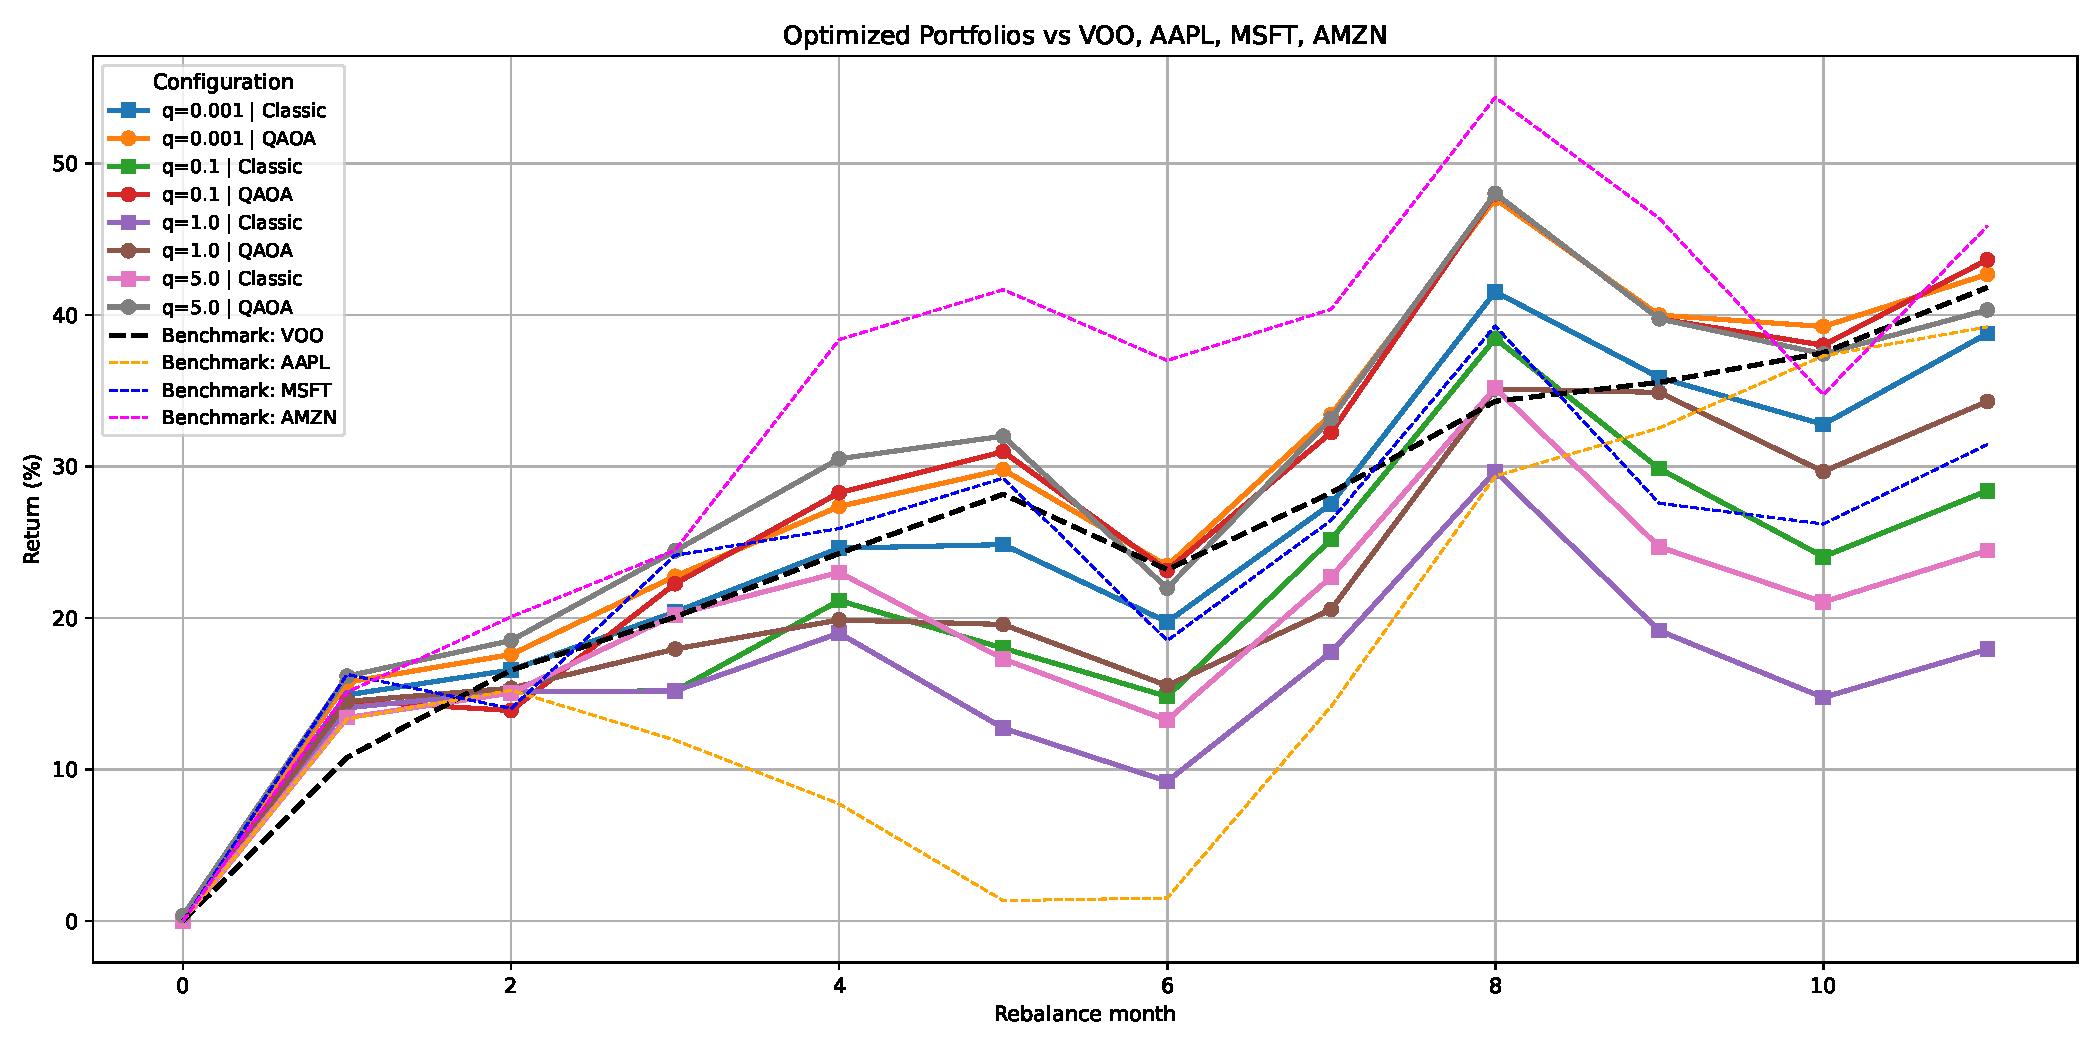
\includegraphics[width=1.0\textwidth]{figures/_VOO_bb_bull_study_post.pdf}
    \caption{Return (\%) for AAPL, MSFT, AMZN, and VOO versus optimized portfolios from 2023-10-27 to 2024-10-24 (bull market). The optimization used $\lambda_{1} = 1000$ with an initial \$10{,}000 investment, rebalanced every 21 days without additional contributions.}
    \label{fig:VOO_bb_bull_study}
\end{figure}

The bull market from October 2023 to October 2024 provided an ideal environment to assess the responsiveness and return-capturing capabilities of the portfolio optimization strategies. During this upward-trending period, all portfolios benefited from broad-based equity appreciation; however, the portfolios optimized using the Quantum Approximate Optimization Algorithm (QAOA) outperformed their classically optimized counterparts across most configurations.

Notably, QAOA portfolios with lower risk-aversion parameters (\( q = 0.001 \) and \( q = 0.1 \)) achieved the highest cumulative returns among all strategies, surpassing even the VOO benchmark. These portfolios exhibited sharper growth trajectories and demonstrated the ability to dynamically adjust weights in response to emerging market momentum.

By contrast, the classically optimized portfolios displayed slower return accumulation and more conservative rebalancing behavior, particularly for higher \( q \) values such as \( q = 1.0 \) and \( q = 5.0 \). While these strategies maintained stability, they were less agile in capitalizing on the sustained rally, which led to lower terminal performance. Even at elevated \( q \), QAOA remained competitive, further highlighting its advantage in capturing directional market signals during expansionary phases.

\subsection{Bear market - 2022-01-03 to 2023-01-05}

Following the same reference \cite{fidelity_bear_bull}, a bear market is defined as a drop of 20\% or more from a recent high. For this study, we analyze the ETF VOO, which fell from \$418.825 on 2022-01-04 to \$307.223 on 2022-10-13 — a decline of 26.65\%. Using the same 21-business-day rebalancing frequency and lookback window, we constructed the schedule below. The optimization is performed with a training period of 21 prior trading days, a rebalance interval of 21 days, and a penalty parameter of \(\lambda_1 = 1000\).

\begin{table}[H]
\centering
\caption{Portfolio Rebalancing Schedules}
\begin{tabular}{|l|p{4cm}|p{5cm}|}
\hline
\textbf{Rebalancing Frequency} & \textbf{Description} & \textbf{Rebalancing Dates} \\
\hline
Every 21 business days & \makecell[l]{Monthly\\rebalancing} & 
\makecell[l]{
2022-01-04, 2022-02-03,\\
2022-03-07, 2022-04-05,\\
2022-05-05, 2022-06-06,\\
2022-07-07, 2022-08-05,\\
2022-09-06, 2022-10-05
} \\
\hline
\end{tabular}
\label{tab:bear_VOO}
\end{table}

The bear market spanning January 2022 to January 2023 imposed considerable stress on all portfolios and presented a markedly different set of optimization challenges. In this more volatile and contractionary environment, the QAOA-optimized portfolios once again exhibited superior performance relative to classical methods. Portfolios configured with \( q = 0.001 \) and \( q = 0.1 \) showed higher robustness, managing to track the VOO benchmark more closely and mitigating downside risk more effectively.

The quantum-enhanced portfolios adapted more quickly to transient recoveries within the downtrend and exhibited smoother drawdown profiles.

In contrast, classical solvers—especially with higher \( q \) values—tended to over-penalize deviations from target allocations, resulting in less responsive portfolios. These strategies showed flatter return curves and failed to capture intermediate gains, ultimately lagging both QAOA portfolios and the benchmark. The performance gap was particularly evident during mid-horizon rebalancing steps, where QAOA portfolios rebounded earlier and more sharply.

\begin{figure}[H]
    \centering
    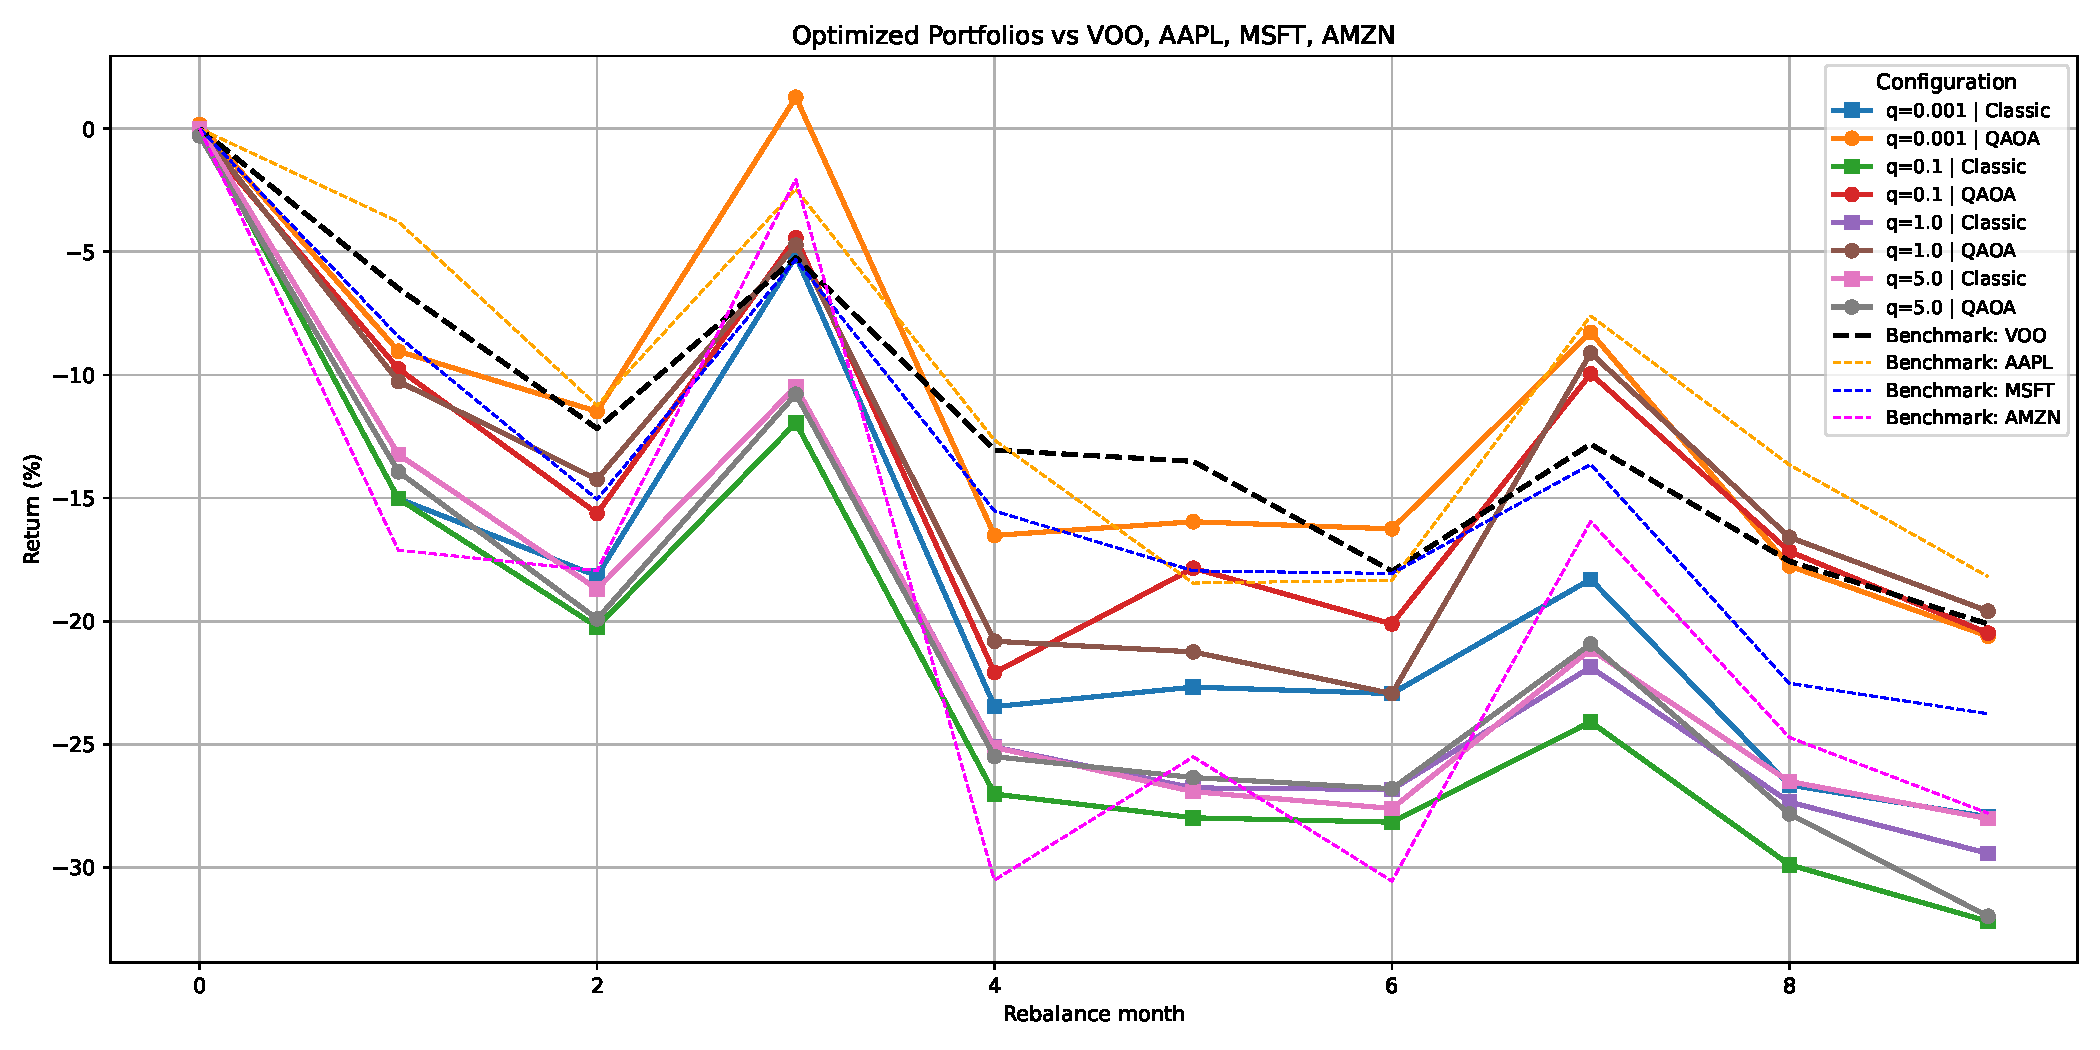
\includegraphics[width=1.0\textwidth]{figures/_VOO_bb_bear_study_post.pdf}
    \caption{Return (\%) for AAPL, MSFT, AMZN, and VOO versus optimized portfolios from 2022-01-03 to 2023-01-05 (bear market). The optimization was performed with $\lambda_{1} = 1000$ on a \$10{,}000 initial investment, without additional capital added at each 21-day rebalance interval.}
    \label{fig:VOO_bb_bear_study}
\end{figure}

\subsection{Bull Market — 2023-10-27 to 2024-10-24 with Additional Investment}

In this analysis, an additional \$1{,}000 USD is added at each 21-day rebalancing step to simulate systematic capital deployment during the bull market. This setup evaluates how classical and QAOA optimization strategies capitalize on sustained market growth under consistent capital inflow. The optimization is performed with a training period of 21 prior trading days, a rebalance interval of 21 days, and a penalty parameter of \(\lambda_1 = 1000\).

\begin{figure}[H]
    \centering
    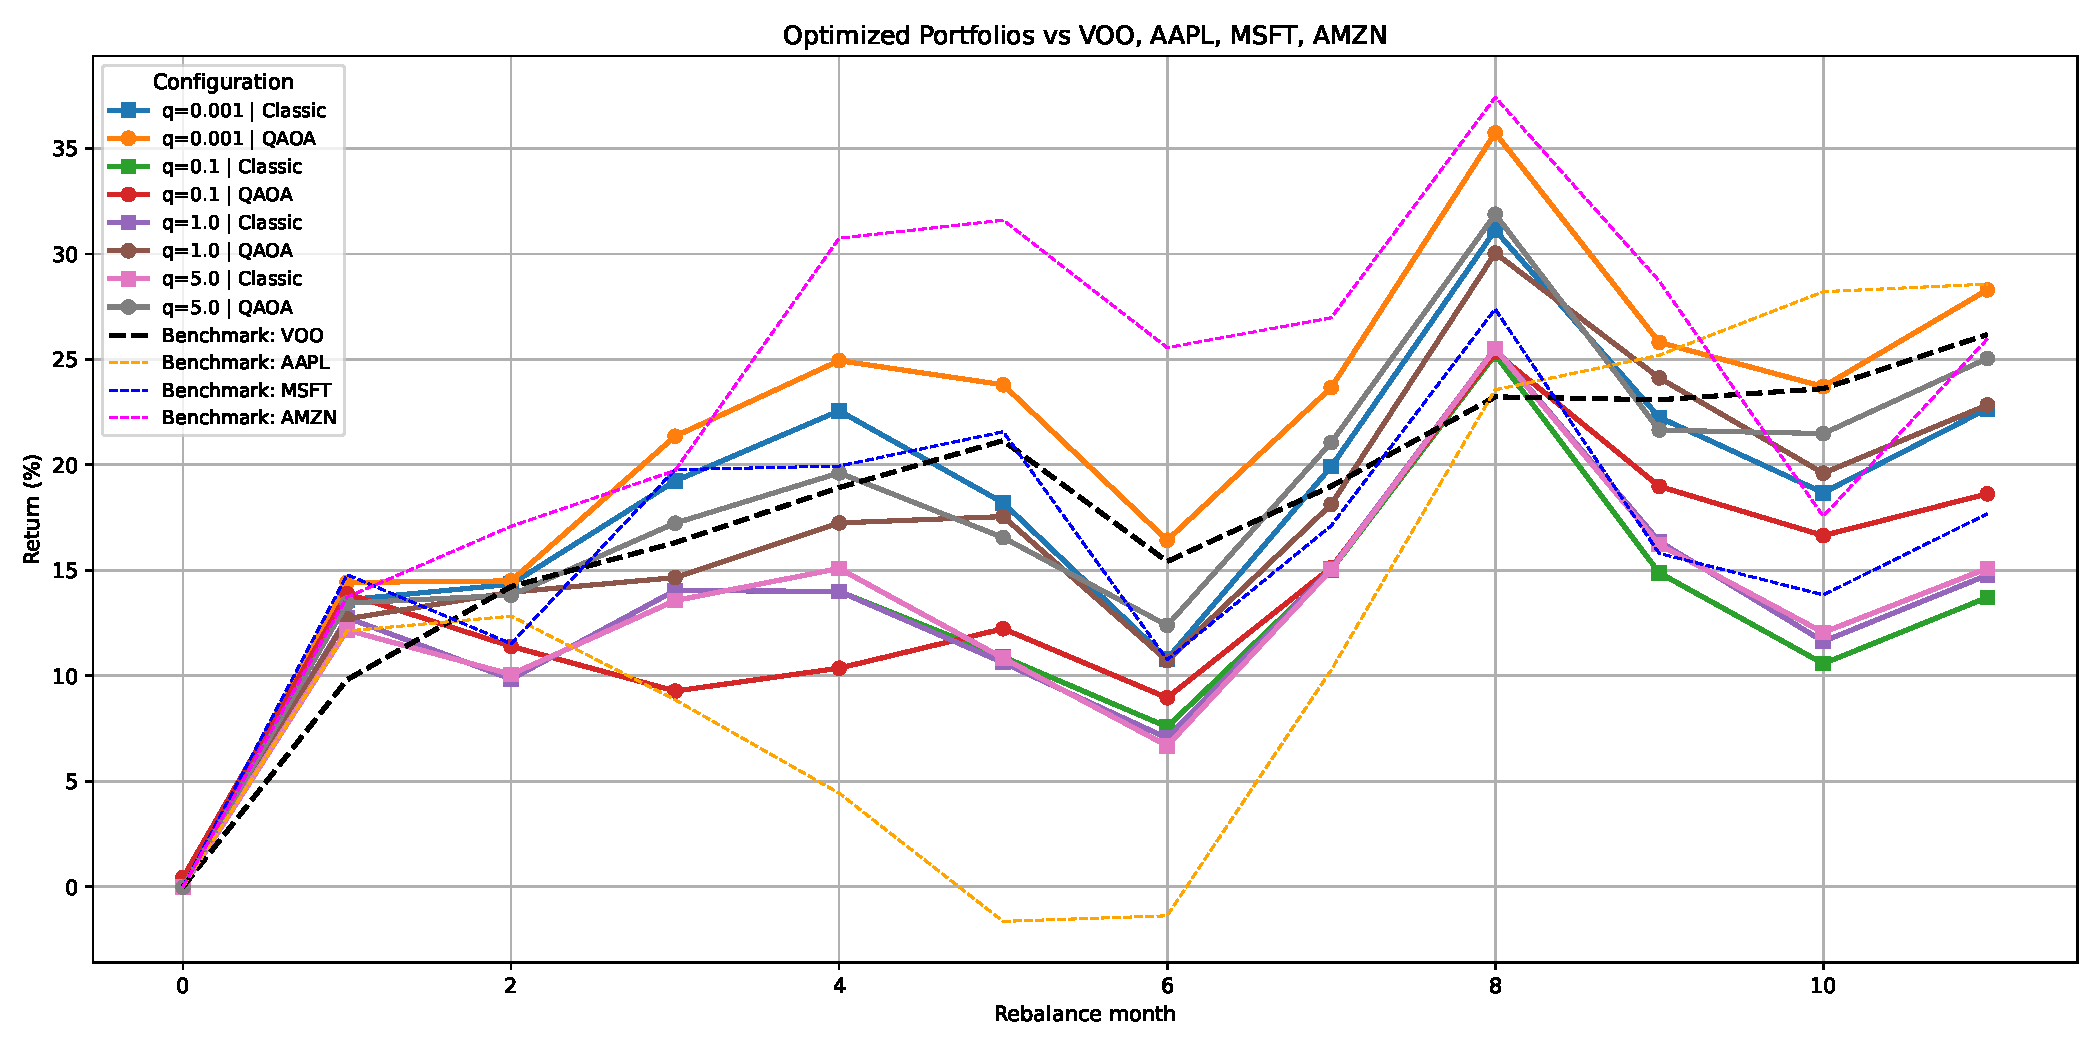
\includegraphics[width=1.0\textwidth]{figures/_VOO_bb_bull_study_post_new_invest.pdf}
    \caption{Return (\%) for AAPL, MSFT, AMZN, and VOO versus optimized portfolios from 2023-10-27 to 2024-10-24 (bull market). The optimization used $\lambda_{1} = 1000$ with an initial \$10{,}000 investment, rebalanced every 21 days with \$1{,}000 additional contributions each rebalance period.}
    \label{fig:VOO_bb_bull_study_new_invest}
\end{figure}

In the bull market setting, all portfolios—whether optimized classically or via QAOA — experienced positive returns. However, QAOA-optimized portfolios consistently outperformed their classical counterparts across all levels of the risk aversion parameter \( q \). The performance gap is especially pronounced at lower values, where the QAOA portfolio with \( q = 0.001 \) achieves the highest overall return among all configurations. This suggests that QAOA's hybrid optimization scheme is more effective in dynamically adjusting to sustained upward trends. Classical portfolios, particularly at higher \( q \) values such as \( q = 5.0 \), exhibit slower growth and fall short of both the benchmark VOO and the corresponding QAOA portfolios. The results indicate that QAOA not only tracks the benchmark more efficiently but also captures additional upside, especially when the risk aversion parameter (\( q \)) is moderate or low. This outcome aligns with our hypothesis that lower risk aversion allows for more flexible deviation from the benchmark, enabling the optimizer to take advantage of high-return opportunities during a sustained market uptrend.


\subsection{Bear Market — 2022-01-03 to 2023-01-05 with Additional Investment}

An additional \$1{,}000 USD is allocated to the portfolio every 21 days during the bear market period, reflecting a strategy of continuous reinvestment under adverse conditions. The analysis compares how classical and QAOA solvers respond to ongoing capital injections and manage drawdown risk in a declining market. The optimization is performed with a training period of 21 prior trading days, a rebalance interval of 21 days, and a penalty parameter of \(\lambda_1 = 1000\).

\begin{figure}[H]
    \centering
    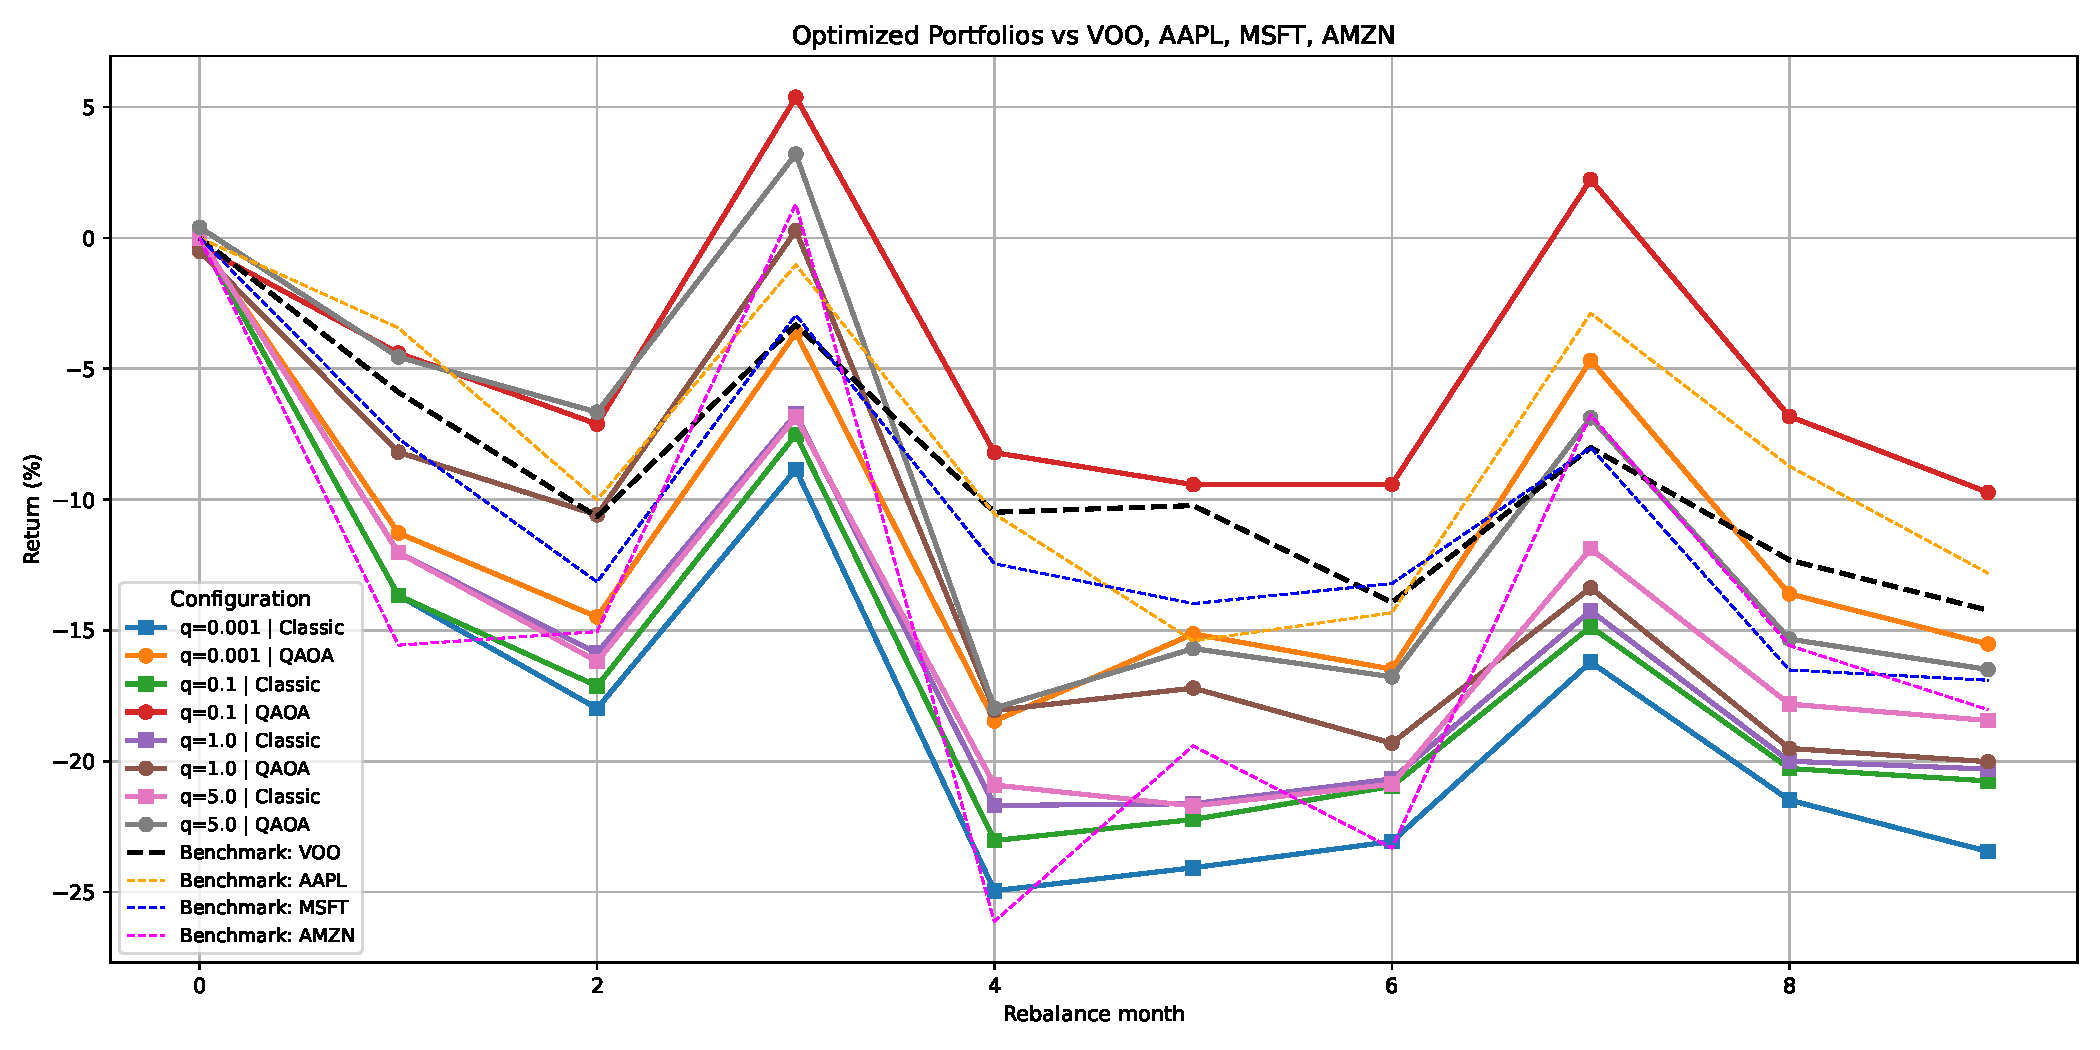
\includegraphics[width=1.0\textwidth]{figures/_VOO_bb_bear_study_post_new_invest.pdf}
    \caption{Return (\%) for AAPL, MSFT, AMZN, and VOO versus optimized portfolios from 2022-01-04 to 2022-10-13 (bear market). The optimization used $\lambda_{1} = 1000$ with an initial \$10{,}000 investment, rebalanced every 21 days with \$1{,}000 additional contributions each rebalance period.}
    \label{fig:VOO_bb_bear_study_new_invest}
\end{figure}

During the bear market period, returns were generally lower across all portfolios, yet the QAOA-optimized configurations consistently outperformed their classical counterparts. Notably, QAOA with low risk aversion parameters (\( q = 0.001 \) and \( q = 0.1 \)) maintained closer alignment with the VOO benchmark and exhibited more resilient return profiles under adverse conditions. In contrast, classical methods—particularly at higher levels of \( q \)—produced flatter trajectories and diverged more significantly from the benchmark over time. The comparatively stronger performance of QAOA in this regime suggests that its hybrid quantum-classical optimization framework adapts more effectively to sustained drawdowns and transient market rebounds. Even under persistent stress, QAOA demonstrated the ability to contain losses and exploit short-term recoveries more efficiently than classical solvers.


\section{Conclusion}

This study compares quantum and classical portfolio optimization strategies across bull and bear market regimes, under both static and dynamically growing capital scenarios. Overall, QAOA consistently outperforms classical Numpy-based optimization, particularly when configured with low risk aversion parameters (\( q = 0.001 \) and \( q = 0.1 \)). These QAOA configurations maintain closer tracking to the VOO benchmark and demonstrate more resilient return profiles during market downturns, while also achieving superior growth in bullish conditions. 

In scenarios without additional investment, QAOA still preserves a performance edge by effectively navigating volatile return surfaces. When periodic capital injections are introduced, QAOA portfolios more efficiently allocate new funds to exploit market momentum or cushion losses. In contrast, classical optimization methods generally exhibit lower overall returns and are more prone to underperformance during drawdowns, particularly at higher \( q \) values. These findings highlight QAOA's adaptability and its potential value as a forward-looking tool for dynamic portfolio management under varying market conditions.

\section{Future Work}

Future work will incorporate transaction costs, multiple asset classes, and extended constraints to better reflect realistic investment scenarios. Additionally, given the memory limitations of current quantum simulators, future experiments will aim to access real quantum hardware to fully explore QAOA’s potential at scale.

\printbibliography
\end{document}
